\def\UnicodeFontFile#1#2{"[../fonts/#1.otf]:#2"}
\input{tulmr.fd}
\documentclass[11pt,a4paper]{article}
\usepackage[margin=22mm,headheight=14pt,footskip=12mm]{geometry}
\usepackage{fontspec}
\defaultfontfeatures{Path=../fonts/}
\usepackage{unicode-math}
\setmathfont{latinmodern-math.otf}
\usepackage{amsmath,booktabs,longtable,array,calc,graphicx,xcolor}
\usepackage{microtype,ragged2e,enumitem,seqsplit,etoolbox}
\usepackage{newunicodechar,float}
\usepackage{pid-rs-report-tables}
\usepackage{pid-rs-workflow-publication}
\usepackage{hyperref,xurl,bookmark}
\pdfvariable minorversion=7
\pdfvariable suppressoptionalinfo=767
\pdfextension catalog { /Lang (en) }
\hypersetup{colorlinks=true,linkcolor=PidPrimary,urlcolor=PidSecondary,citecolor=PidSecondary,filecolor=PidSecondary,pdftitle={Wibral-line PID for physical intelligence},pdfauthor={Sepehr Mahmoudian},pdfsubject={Results, limits and the next sensor experiment},pdfdisplaydoctitle=true}
\PidSetRunningHeads{Categorical shared exclusions}{Embodied sensor utility}
\PidWorkflowConfigureSections
% Compose unavailable text glyphs in the current text family, including inline code.
\newunicodechar{₂}{\textsubscript{2}}
\newunicodechar{≈}{\ensuremath{\approx}}
% Keep each admitted figure in its source order.
\floatplacement{figure}{H}
\setcounter{secnumdepth}{0}
\setlength{\parindent}{0pt}
\setlength{\parskip}{0.48em plus 0.10em minus 0.06em}
\setlength{\emergencystretch}{3em}
\setlength{\LTpre}{0.5em}
\setlength{\LTpost}{0.5em}
\setlist{itemsep=0.2em,topsep=0.3em}
\raggedbottom
\clubpenalty=10000
\widowpenalty=10000
\providecommand{\tightlist}{\setlength{\itemsep}{0pt}\setlength{\parskip}{0pt}}
\providecommand{\pandocbounded}[1]{#1}
\providecommand{\passthrough}[1]{#1}
\setkeys{Gin}{width=\linewidth,keepaspectratio}
\newcounter{none}
\let\PidSavedTexttt\texttt
\renewcommand{\texttt}[1]{\PidSavedTexttt{#1}}
\AtBeginEnvironment{longtable}{\footnotesize\RaggedRight\setlength{\tabcolsep}{3pt}}
\title{\PidReportTitle{Wibral-line PID for physical intelligence}{Results, limits and the next sensor experiment}}
\author{Sepehr Mahmoudian}
\date{23 September 2026}
\begin{document}
\microtypesetup{expansion=false}
\RaggedRight
\PidMakeTitle
The immediate application is \textbf{offline sensor analysis for embodied prediction}: two cameras, with optional audio, used to predict a separately measured future physical outcome. This is an attainable first step toward robust world models and robot policies. It is not yet a demonstrated training or control improvement.

The selected functional is \textbf{Makkeh--Gutknecht--Wibral categorical shared exclusions (MGW)}, in nats, with signed atoms. The \href{https://arxiv.org/abs/2002.03356v5}{defining paper} is distinct from continuous shared exclusions and from other PID definitions. Fitted bins define a categorical estimand; raw sensor information is a different object.

\par\Needspace{10\baselineskip}

\section{The practical finding}\label{the-practical-finding}

An extra sensor's value is not its synergy alone. For two-source atoms \(R,U_1,U_2,S\), the added Shannon information is \(U_2+S\). If source 1 is available with probability \(a\) and source 2 with probability \(b\), with availability indicators \(M_1,M_2\) such that \(M_1\perp M_2\) and \((M_1,M_2)\perp(X_1,X_2,Y)\), the added Bayes log-loss value is

\[
\Delta=b[(1-a)R+U_2+aS].
\]

Both predictors must see the same mask, and the complete-data policy and target law must remain fixed. Redundancy can provide backup value; unique information and synergy combine when sensors are present. The full proof includes correlated failures and data-dependent missingness in the \href{https://github.com/sepahead/pid-rs/blob/main/output/pdf/embodied-sensor-utility.pdf}{detailed report}.

For independent fair bits \(A,B,U\), set the same target \(Y=(A,B)\) and baseline \(X_1=A\). Candidate noise \(U\) and useful complement \(B\) both have MGW synergy \(\ln(4/3)\). Their added information is respectively zero and \(\ln2\). A duplicate \(A\) has zero synergy but supplies backup value when the first copy is unavailable.

\begin{figure}
\centering
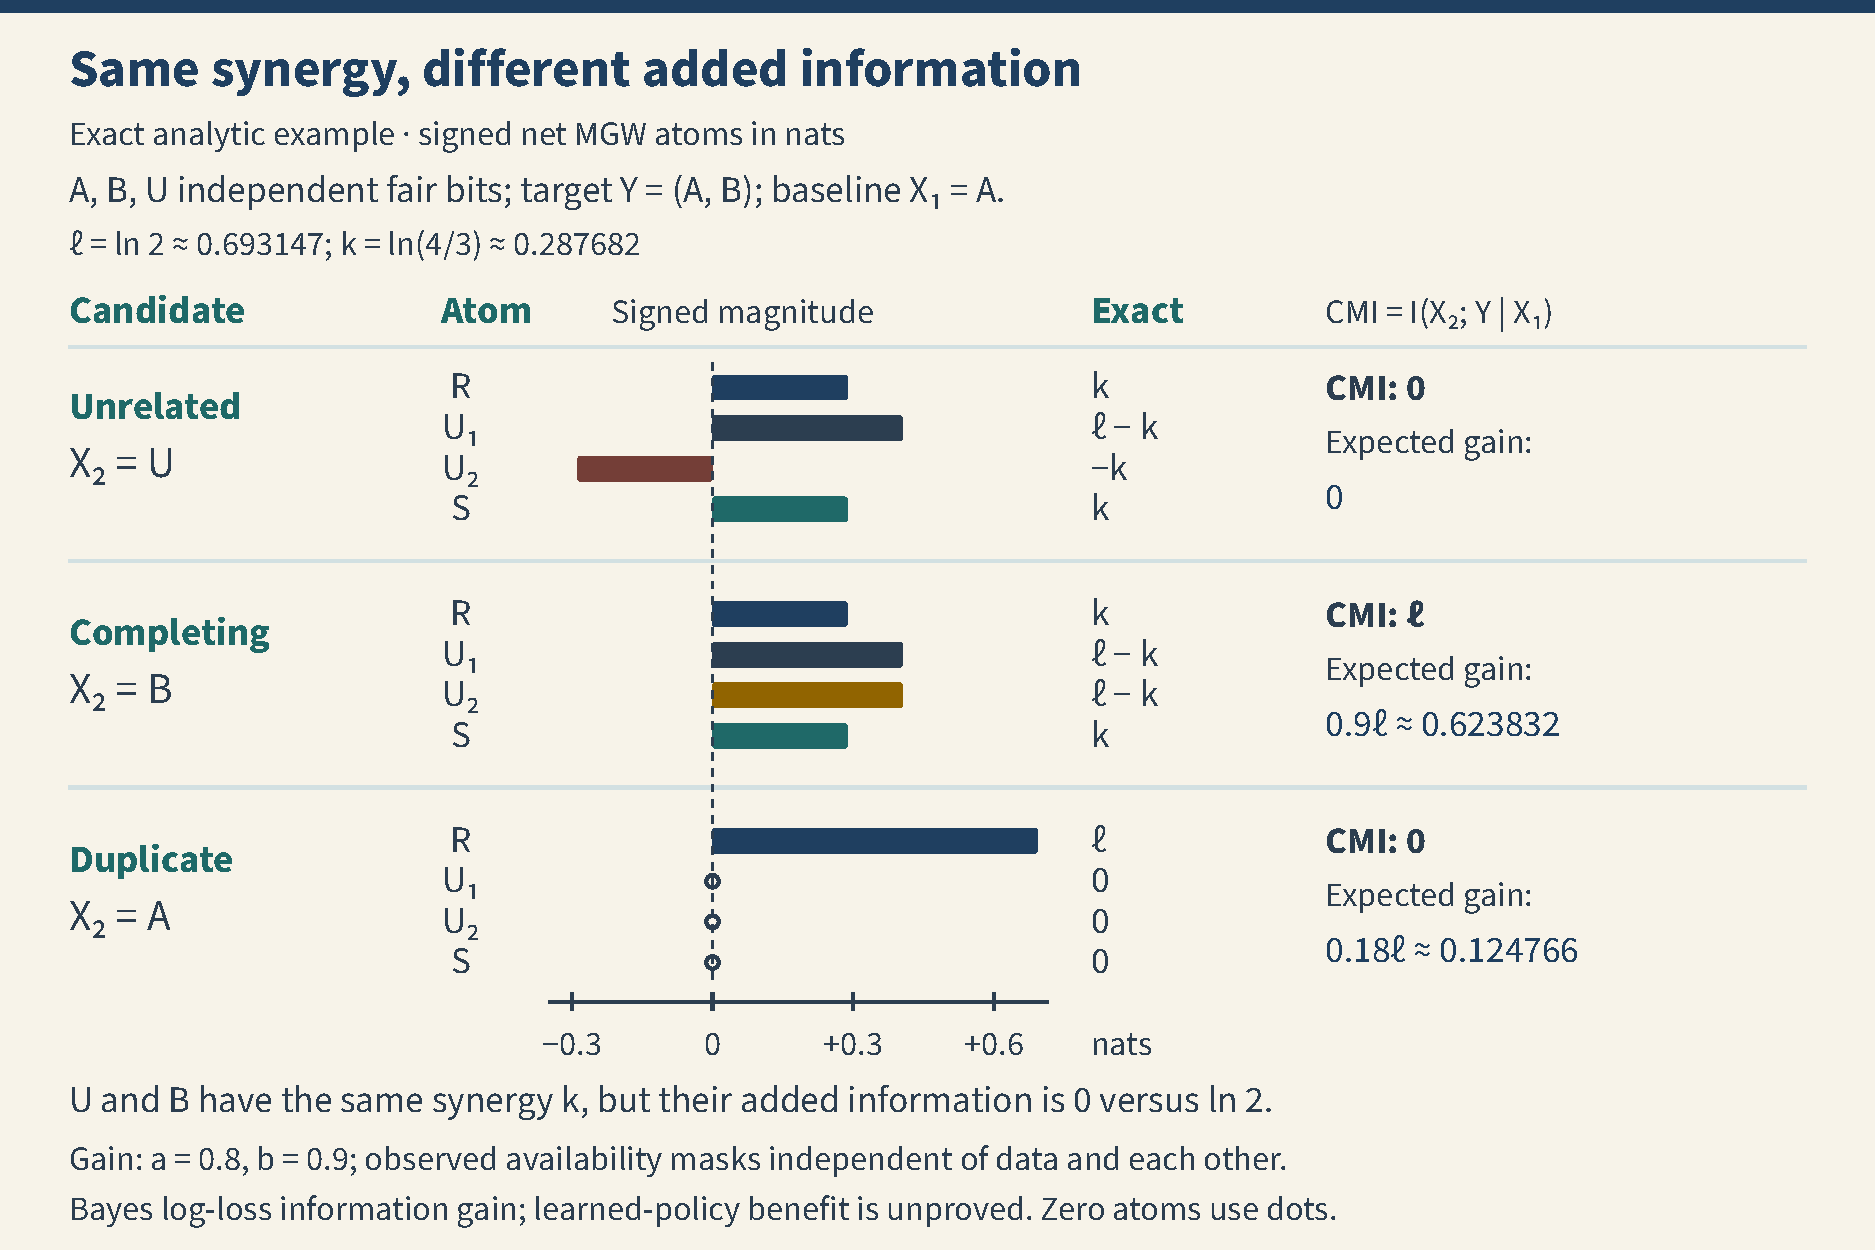
\includegraphics[width=160mm,height=\textheight,keepaspectratio,alt={One target law, three candidate sensors. Signed unique information distinguishes noise from a useful complement despite equal synergy; duplication can have backup value.}]{figures/signed-atoms-and-sensor-value.pdf}
\caption{One target law, three candidate sensors. Signed unique information distinguishes noise from a useful complement despite equal synergy; duplication can have backup value.}
\end{figure}

There is also a useful limit: the expected Bayes log-loss reduction relative to the no-source predictor, under a fixed law and exogenous availability, depends only on subset mutual information. For two to four sources, that is 3, 7 or 15 values. Full PID's 4, 18 or 166 atoms provide a finer allocation, but no extra decision information for that exact objective. PID must earn additional cost through a useful diagnostic question or a separately justified objective.

\par\Needspace{10\baselineskip}

\section{What exists and what it supports}\label{what-exists-and-what-it-supports}

{\def\LTcaptype{none} % do not increment counter
\begin{longtable}[]{@{}
  >{\raggedright\arraybackslash}p{(\linewidth - 4\tabcolsep) * \real{0.2800}}
  >{\raggedright\arraybackslash}p{(\linewidth - 4\tabcolsep) * \real{0.3200}}
  >{\raggedright\arraybackslash}p{(\linewidth - 4\tabcolsep) * \real{0.4000}}@{}}
\toprule\noalign{}
\begin{minipage}[b]{\linewidth}\raggedright
Work
\end{minipage} & \begin{minipage}[b]{\linewidth}\raggedright
Useful role
\end{minipage} & \begin{minipage}[b]{\linewidth}\raggedright
Remaining boundary
\end{minipage} \\*
\midrule\noalign{}
\endhead
\bottomrule\noalign{}
\endfoot
Rust categorical MGW for 2--4 sources & Offline signed atom calculation with budgets and cancellation & No completed sensor benchmark follows from library availability \\*
\href{https://github.com/sepahead/pid-rs/blob/main/audit/formal/lean-finite-logscore/PUBLICATION.md}{Four classical finite-PMF foundations} & Mass/measure, integral, Gibbs and log-score results checked locally in Lean & Unconditional law only; 13 downstream conditional sensor/application targets remain open \\*
Equal-synergy and target-copy formal work & Reject an invalid synergy-only selection rule & Exact theorem premises and replay status remain in the theorem maps \\*
Fixed-alphabet continuity and dependence-aware law bounds & Conditional tools for estimator sensitivity & A valid sampling/dependence model is still required \\*
Finite-prefix mean, bias and gradient work & Mathematical tools for a future bounded encoder experiment & Not an implemented robot-training method \\*
Availability exposition & Complete classical derivation, controls and experiment design & Conditional prediction and availability/mask arguments remain handwritten; no scientific-priority claim \\*
\end{longtable}
}

The \href{https://github.com/sepahead/pid-rs/blob/main/MATHEMATICAL_RESULTS_GUIDE.md}{mathematical results guide} points to standalone proofs and exact formal status. A verified mathematical intermediate step does not establish estimator calibration or physical value.

\par\Needspace{10\baselineskip}

\section{Rust implementation and computational cost}\label{rust-implementation-and-computational-cost}

Rust supplies budgeted categorical MGW for two to four sources through the \href{https://github.com/sepahead/pid-rs/blob/main/crates/pid-core/src/lib.rs}{averaged API}. Event calculations are quadratic in the occupied complete states \(K\) for each lattice node. Averaged output saves retained pointwise results; row and PMF storage remain. Dense log-score validation and evaluation over \(K_Y\) target labels take \(O(K_Y)\) work and \(O(1)\) extra storage beyond the inputs.

No Rust log-score evaluator or learner is added; floating-point execution is unverified. Feature extraction, masked prediction, training and resampling add costs. Begin offline: latency and learning benefit are unmeasured. See the \href{https://github.com/sepahead/pid-rs/blob/main/audit/research/embodied-sensor-utility/EXPOSITION.md\#13-rust-implementation-and-computational-cost}{full cost discussion}.

\par\Needspace{10\baselineskip}

\section{The ecosystem connection}\label{the-ecosystem-connection}

CREBAIN produces observations; NCP transports sensor records; Prisoma inspects experiments; pid-rs computes information; Galadriel can retain diagnostic evidence. Manwe supplies a separate tracking setting. The detailed report distinguishes existing consumers from proposals.

The current two-camera-plus-audio example records five images and 800 pressure samples over six 120-Hz body ticks. That proves a capture composition, not independent statistical replication. The missing step is a frozen feature table joined to future reference labels. Use one declared episode/landmark unit, preserve timing and missingness, fit transforms only on training episodes, and evaluate untouched episodes.

\par\Needspace{10\baselineskip}

\section{How practical value will be tested}\label{how-practical-value-will-be-tested}

Start offline with all eight sensor subsets. Measure predictive loss, availability, runtime and memory. Keep fixed-model outages separate from retrained subset models. Compare MI/CMI, subset task loss and established masking methods. \href{https://proceedings.mlr.press/v270/skand25a.html}{Masked sensor training} and \href{https://proceedings.mlr.press/v305/almuzairee25a.html}{MAD multi-view reinforcement learning} are relevant baselines; no superiority to them is established here.

The detailed report derives a conservative paired-episode loss bound and states its independence and bounded-probability assumptions. It also explains why natural occlusion needs conditional laws, why more sensors can defeat finite-data estimation, and why an action-conditioned latent must not be evaluated against its own injected action.

Testing control, placement or re-identification requires explicit target, policy, association and cost contracts. Require useful task gains against matched baselines and retain negative results.

\textbf{How to cite:} Sepehr Mahmoudian, \emph{Wibral-line PID for physical intelligence}, pid-rs technical report, 2026. Include the exact repository commit or release. Use the \href{https://github.com/sepahead/pid-rs/blob/main/CITATION.cff}{citation metadata} for the software and cite the defining method papers separately.
\end{document}
